%%%%%%%%%%%%%%%%%%%%%%%%%%%%%%%%%%%%%%%%%%%%%%%%%%%%%%%%%%%%%%%%%%%
%                                                                 %
%                            CHAPTER FIVE                         %
%                                                                 %
%%%%%%%%%%%%%%%%%%%%%%%%%%%%%%%%%%%%%%%%%%%%%%%%%%%%%%%%%%%%%%%%%%%

\chapter{Data Volatility}

\section{Introduction}

Capturing change counts is important but understanding how a data set changes over time is also valuable to users.

Look at Figure \ref{GCMDC1} and notice the different total amounts of change in each version of GCMD Keywords.
The group appears to do significantly less work in updating the data set after Version 8.1, but the appearance only occurs because the versions are disconnected from time.
Once we're able to quantify change, we can begin looking at trends over time.
Data volatility is the likelihood or rate of data change.
Volatility helps explain the 
We want to know if data versions are hiding the actual rate of change

\section{Determining Volatility}

Instead of charting the version changes in evenly wide bars, the versions are spread across time based on the time of publication to the KMS as seen in Figure \ref{GCMDPlot1}.
\begin{figure}%[b]
	\centering
	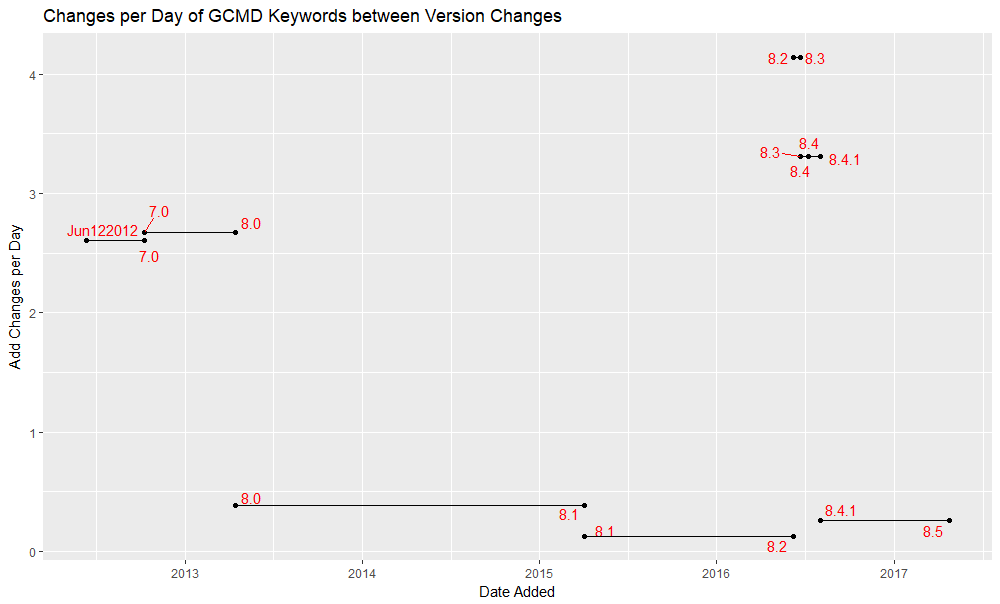
\includegraphics[scale=0.56]{figures/GCMDPlot1.png}
	\caption[Global Change Master Direcotry counts distributed over time.]{Add counts for all versions of GCMD up to 8.5 evenly distributed over the time of version validity.}
	\label{GCMDPlot1}
\end{figure}
Since each of the versions were dominated by the \textbf{Add} counts, the count is divided by the number of days between the publication of a version on the left side of the line and the release of the replacement version on the right side of the line.
The height of the line on the chart gives the steady rate of change until the release of the new version.
The area underneath the line is the total amount of change the new version introduces.
Since each version packages together all the changes into a single release, the actual change rate is unknown.

Three observable clusters appear in the time aware presentation of the versions, highlighted in Figure \ref{GCMDPlot1Cluster}.
\begin{figure}%[b]
	\centering
	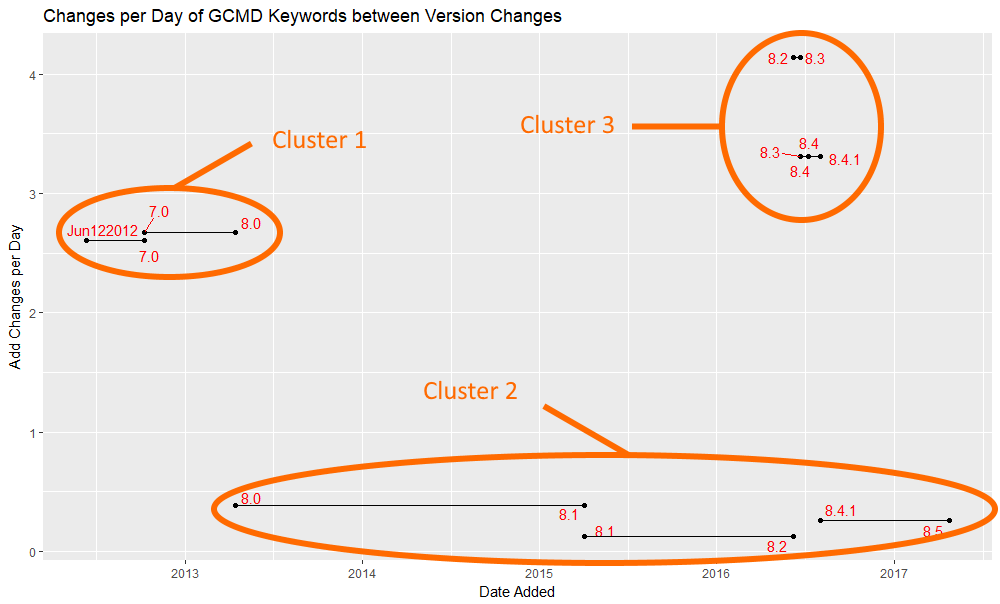
\includegraphics[scale=0.56]{figures/GCMDPlot1_Cluster.png}
	\caption[Global Change Master Directory count distributed over time with clusters marked.]{The change rate of different versions organize into three visible clusters. Cluster 2 denotes a sudden burst of version releases which is notable.}
	\label{GCMDPlot1Cluster}
\end{figure}
According to the Keyword Governance and Community Guide Document \cite{gcmd_gov}, ``Full GCMD keywords list releases get a new major version number (e.g., 8.0). Incremental releases for updates to topics, terms, and variables get a new minor version number (e.g., 8.1).”
The statement explains the activity in Cluster 1 where there are sufficient changes to warrant a full release of the keywords.
Cluster 2 captures the change rate and duration of minor versions, except those from 8.2 to 8.4.1 which are in Cluster 3.
Cluster 3 demonstrates a flurry of activity occurring between June 7, 2016, to August 2, 2016.
Considering the previous pattern of taking at least six months between releases, three minor version releases within as many months is highly unusual.

An immediate concern is that Cluster 3 does not result from a sudden burst of activity, necessitating rapid version replacement.
An inquiry into reasoning behind the successive publication returned a statement that the government customer had requested the action.
Another way to dig into the behavior is to look into the impact assessments accompanying the versions.
Impact assessments prior to Version 8.5 are not publicly available, and only assessments for versions 8.2, 8.3, and 8.4 were received upon request.
Of the 6 requests affecting Earth Science Keywords in 8.2, published June 7, 2016, 4 were made in 2014, and the remaining 2 were made in 2015.
Version 8.3 had 8 entries in its impact assessment with 7 entries originating in 2014, and the remaining entry from 2015.
The 6 entries 8.4’s impact assessment has 5 entries from 2008 and 1 entry from 2015.
The data is collected in Table \ref{table:GCMD_old}.
\begin{table}
	\caption{Global Change Master Directory versions with old start time changes.}
	\label{table:GCMD_old}
	\centering
	\begin{tabular}{|c|c|c|c|c|}
		\hline
		Version Name&	Publish Date&	2008&	2014&	2015\\ \hline
		8.2&	June 7, 2016&	0&	4&	2\\
		8.3&	June 21, 2016&	0&	7&	1\\
		8.4&	July 7, 2016&	5&	0&	1\\
		\hline
	\end{tabular}
\end{table}


\section{Earth Observing Laboratory}

The Earth Observing Laboratory (EOL) of the National Center for Atmospheric Research (NCAR) distributes small data sets, around 10-12 files per data set, regarding lower atmospheric data beginning in 2005 \cite{EOL}.
The EOL data sets are somewhat unique in the data set size means management often does not require automation.
In mid-2014, EOL began assigning versions to stored data sets.
When receiving a new version of a data set from a researcher, the practice is to upload the entire new data set, and replace all old files.

Of the 1335 data sets maintained by EOL with versions, only 180 data sets had more than one version.  
The full distribution of version counts is in Table \ref{table:EOL_Versions}
\begin{table}
	\caption{Version Content of Earth Observing Laboratory Data Sets}
	\label{table:EOL_Versions}
	\centering
	\begin{tabular}{|c|c|}
		\hline
		Number of Versions& Number of Data Sets\\ \hline
		1&	1155\\
		2&	141\\
		3&	26\\
		4&	10\\
		5&	3\\
		Total&	1335\\
		\hline
	\end{tabular}
\end{table}
The 1155 other data sets were filtered out since change counts could not be computed for single-version collections.
Since all the files are replaced on an update and a unique file identifier like a hash sum was unavailable, file matching between versions rely on filenames to perform change mappings.
For all files that matched names across versions, the relation was classified as \textbf{Modify}.  
The approach will over-count the number of modifications, but provides an upper bound on the data set volatility in the repository.  
Each count is then normalized by the number of files in the previous version to standardize comparison between data sets regardless of data set size.  
The average for each data set is taken for each change type.

\section{EOL Versioning Behavior}

Given that EOL replaces the entire old data set when updating, the expected behavior of the transitions would be \textbf{Modifies} concentrating close to 1 and \textbf{Adds} and \textbf{Invalidates} distributed close to 0.
The assumption is that researchers have little reason to change the file naming scheme.
The data surprisingly indicates that data sets in EOL primarily gravitate towards \textbf{Addition} and \textbf{Invalidation} values of 1.
\textbf{Modify} counts score more close to 0 in a complete reversal of expectations.

Figure \ref{EOL_Adds} shows the distribution of \textbf{Add} scores.
\begin{figure}%[b]
	\centering
	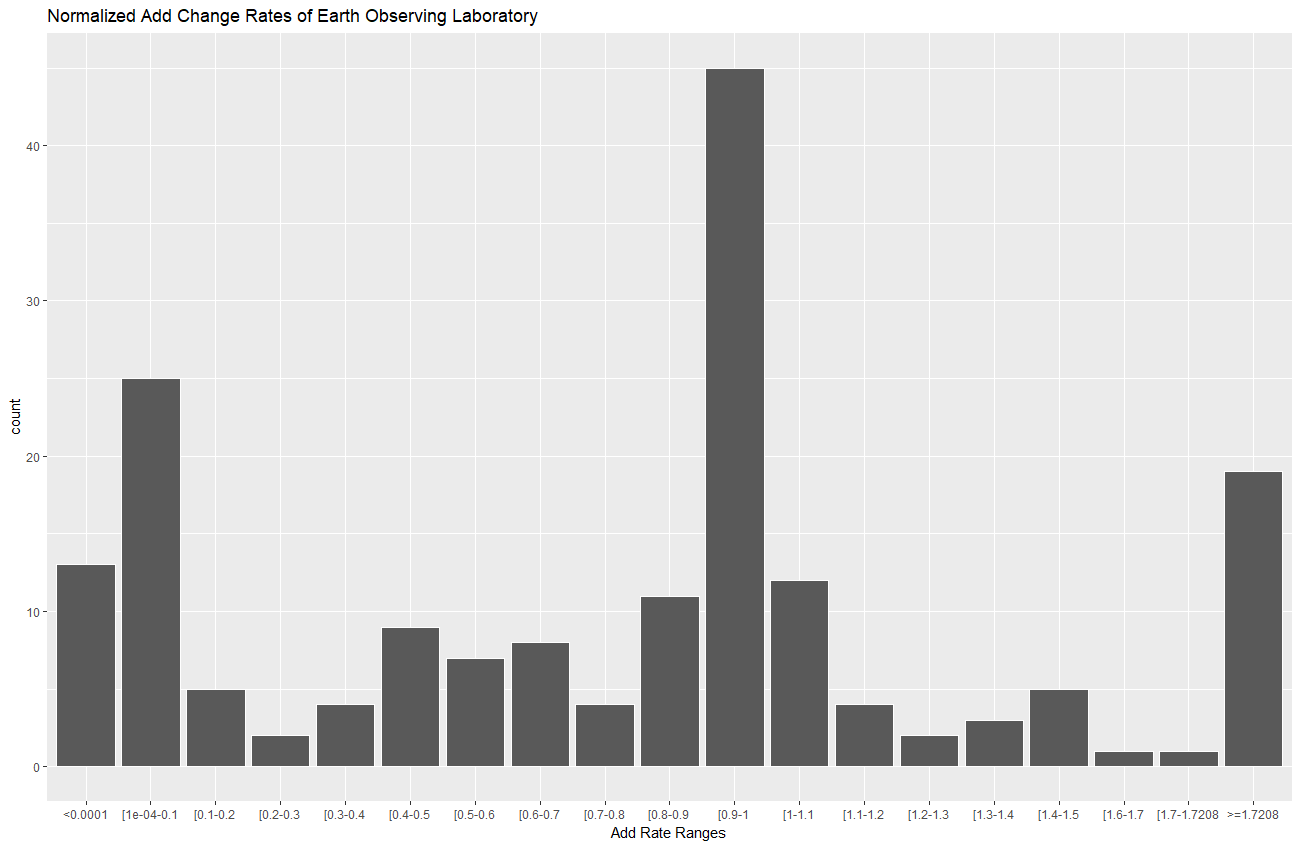
\includegraphics[scale=.43]{figures/Eol_Adds.png}
	\caption{Distribution of average normalized Add counts for each data set in Eath Observing Laboratory.}
	\label{EOL_Adds}
\end{figure}
The primary feature of the chart is the bar situated in the `[0.9-1' range, meaning that about 45 data sets add a number of files equal to the original size of the data set.
Secondary features include the bars on the far right and far left of the chart, but the bar on the right side is a collection of outliers.
In the outlier data sets, the size of the data set increased drastically compared to the behavior of other data sets managed by EOL.
Outliers are determined by collecting values above 1.5 times the interquartile range (IQR) showing in Table \ref{table:EOL_Change}.
\begin{table}
	\caption{Normalized Change Statistics}
	\label{table:EOL_Change}
	\centering
	\begin{tabular}{|c|c|c|c|}
		\hline
		Stat&	Add&	Invalidate&	Modify\\ \hline
		Mean&	0.714312707&	0.654819294&	0.345180706\\
		Std. Dev&	0.509878564&	0.420093557&	0.420093557\\
		Min&	0&	0&	0\\
		Q1&	0.28635075&	0.142857&	0\\
		Med&	0.9146635&	0.9642855&	0.0357145\\
		Q3&	1.00358625&	1&	0.857143\\
		Max&	54.25&	1&	1\\
		IQR&	0.7172355&	0.857143&	0.857143\\
		\hline
	\end{tabular}
\end{table}
A more muted distribution appears around the 0.5 mark where data sets grow more gradually.

The normalized \textbf{Invalidation} score in Figure \ref{EOL_Invs} shows a majority of data sets removing all or almost all files in the data set.
\begin{figure}%[b]
	\centering
	\includegraphics[scale=.6]{figures/Eol_Inv.png}
	\caption{Distribution of average normalized Invalidate counts for each data set in Eath Observing Laboratory.}
	\label{EOL_Invs}
\end{figure}
Coupled with the information that a quarter of the data sets added close to the original data sets' size of files suggests that the entire data set is being replaced.
\textbf{Invalidations} do not have outliers since only files within the data set can be removed.
The data is extremely biased with only 0.04 separating the median and maximum value.
From Table \ref{table:EOL_Change}, at least a quarter of values are 1.
Figure \ref{EOL_Invs} also shows a muted distrubtion around 0.5.

Figure \ref{EOL_Mods}, representing the normalized \textbf{Modify} distribution, is almost a mirror of the \textbf{Invalidation} chart.
\begin{figure}%[b]
	\centering
	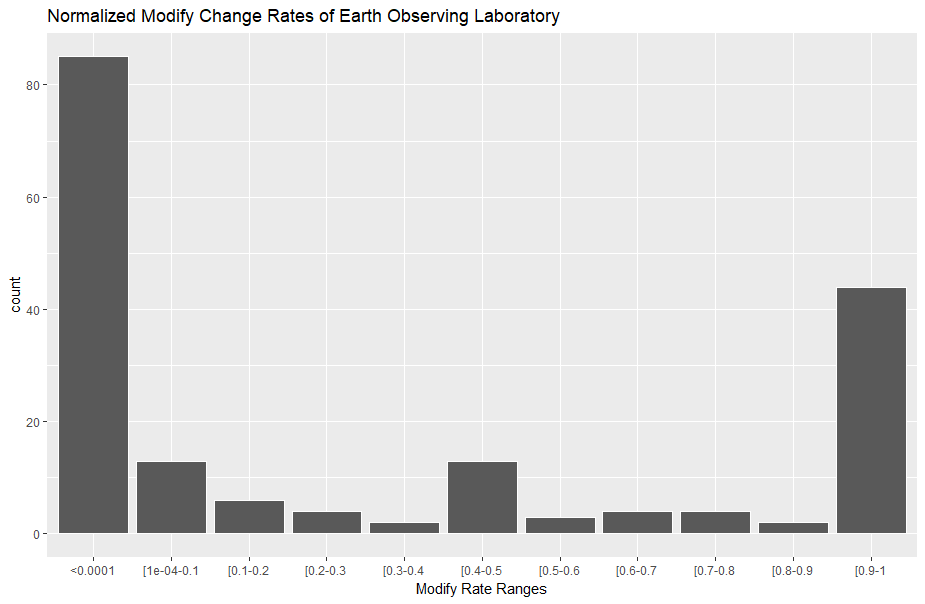
\includegraphics[scale=.6]{figures/Eol_Mod.png}
	\caption{Distribution of average normalized Modify counts of each data set in Eath Observing Laboratory.}
	\label{EOL_Mods}
\end{figure}
The right bar is specifically cut off to capture only 0s, showing that almost a majority of data sets modify 0 files, having 0 files that share names between versions.
The distribution is consistent with a practice of removing all the files in a data set and replacing the files with a new data set using different filenames.
The second feature of this graph shows around 40 data sets in which all or almost all files match across versions.
A small spike of data sets are centralized around 0.5, very much like the other normalized change graphs.

The high concentration of data sets towards 1 in \textbf{additions} and \textbf{invalidations} suggests a more complicated interaction within the data sets.
Individually, the normalized distributions do not show the connection between all three changes since the changes share a common feature, the version transition the changes describe.
Together, the AIM changes create a coordinate in three dimensional space, showing the inter-relation of the changes. 
Figure \ref{EOL_AIM} shows a scatter plot grouping unnormalized change counts for each version.
\begin{figure}%[b]
	\centering
	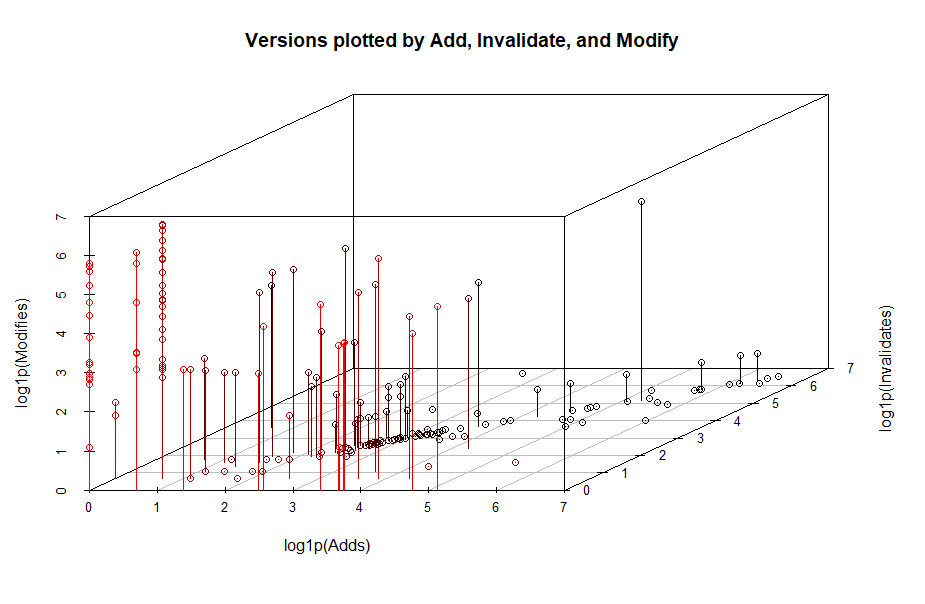
\includegraphics[scale=.6]{figures/Eol_Versions_3d.png}
	\caption{Distribution of average normalized Modify counts of each data set in Eath Observing Laboratory.}
	\label{EOL_AIM}
\end{figure}
Unlike the other charts, the size of the changes are not normalized by data set size, but the values have the log1p function applied to account for a heavy bias towards 12 and 13.
Notice the one-to-one trend between \textbf{Adds} and \textbf{Invalidates} which shows the tendency of data sets to replace every file and assign a new filename.
If the two changes did not co-occur, a normalized \textbf{Add} score of 1 would indicate that data sets tend to double in size instead.
The files are more likely to retain filenames when only a few files in a data set are being modified.

\section{Analysis}

\subsection{Impact Assessment Change Counts}
\begin{table}
	\caption{Differences in VersOn and Impact Assessment metrics}
	\label{table:GCMD_metric}
	\centering
	\begin{tabular}{|r|r|r|r|}
		\hline
		Version & Add & Invalidate & Modify\\ \hline
		8.2(VO)&	53&	1&	26\\
		-8.2(IA)&	48&	0&	4\\
		\hline
		&	\textbf{5}&	\textbf{1}&	\textbf{22}\\
		\hline
		8.3(VO)&	58&	0&	13\\
		-8.3(IA)&	58&	0&	10\\
		\hline
		&	\textbf{0}&	\textbf{0}&	\textbf{3}\\
		\hline
		8.4(VO)&	53&	0&	1\\
		-8.4(IA)&	66&	0&	5\\
		\hline
		&	\textbf{-13}&	\textbf{0}&	\textbf{-4}\\
		\hline
		8.5(VO)&	68&	2&	22\\
		-8.5(IA)&	55&	0&	30\\
		\hline
		&	\textbf{13}&	\textbf{2}&	\textbf{-8}\\						
		\hline
	\end{tabular}
\end{table}

\subsection{Hidden Volatility}

Each version of a data set stored in EOL is assigned three different times, “version publish time,” “version creation time,” and “version modification time.”  
Version publish time indicates the time the version was made available to the public, usually the data set was added to the database.  
Version creation time denotes the moment at which a version designation was given to the collection of files, beginning in mid-2014 when the versioning system was implemented.  
Version modification time indicates the time at which the version metadata was changed.  
Using version publish time most closely resembles the duration of version validity, and the following computations use version publish time.

Some of the data needed to be filtered out to provide valid results.  
Due to a few coding errors in time assignments, 7 versions had to be removed because the durations were negative.  
Duration is measured in days, and the rate of version publication is determined by taking the inverse of the duration.  
To acquire the AIM change rates, the changes are divided by the associated duration for each version.  
Since the rates are closely concentrated at 0, the log of the rates are taken to give the values a more log-normal distribution.  
Values where an AIM change is 0 had to be removed in order to properly apply the log function.  
The remaining number of entries can be found in Table XX.

Since the durations are not normally distributed, but concentrated close to 0, the log of the durations are taken to normalize the data.  
The log function is also applied to the AIM changes to normalize the data.  
The inverse of the log of the duration is taken to acquire the rate of version release.

The Kolomogorov-Smirnov Test was used to determine if the Adds, Invalidates, or Modifies follow a distribution separate from the version publication distribution.  
A difference indicates that the AIM changes exhibit a behavior apart from the version releases.  
As seen in Figures XX, XX, and XX, the distributions of AIM changes over duration are offset due to a larger magnitude of values per version.  
The change rates were translated by the difference in means between the version mean and the associated change mean after log normalization to make the values valid for comparison by the Kolomogorov-Smirnov test.

\begin{figure}%[b]
	\centering
	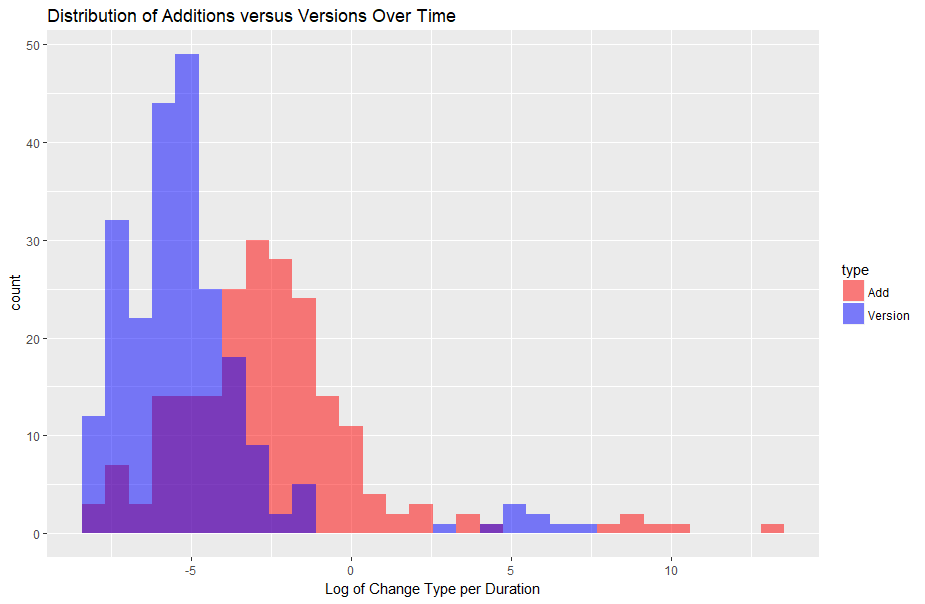
\includegraphics[scale=.6]{figures/Eol_Add_Ver_Rate.png}
	\caption{Distribution of average normalized Modify counts of each data set in Eath Observing Laboratory.}
	\label{EOL_Add_Ver}
\end{figure}

\begin{figure}%[b]
	\centering
	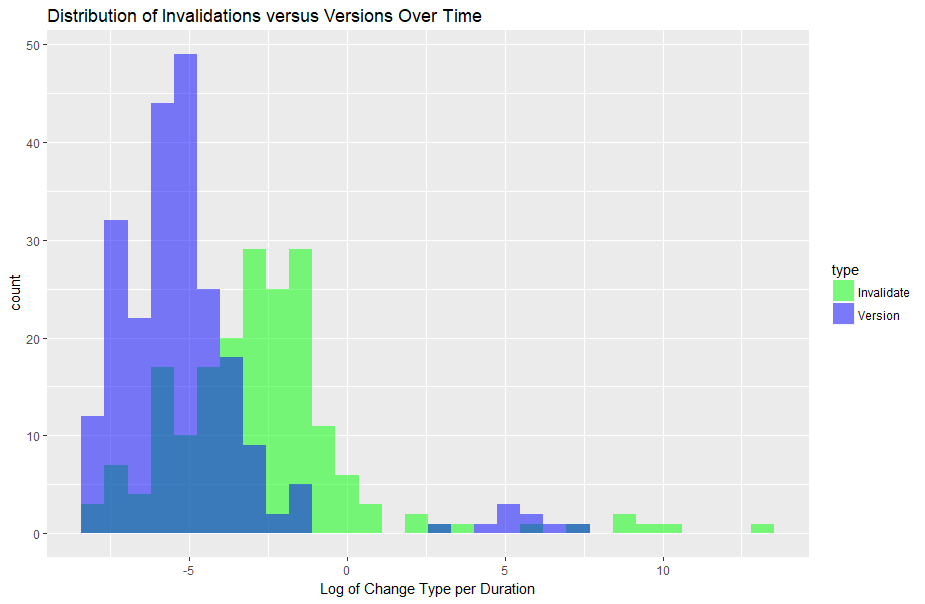
\includegraphics[scale=.6]{figures/Eol_Inv_Ver_Rate.png}
	\caption{Distribution of average normalized Modify counts of each data set in Eath Observing Laboratory.}
	\label{EOL_Inv_Ver}
\end{figure}

\begin{figure}%[b]
	\centering
	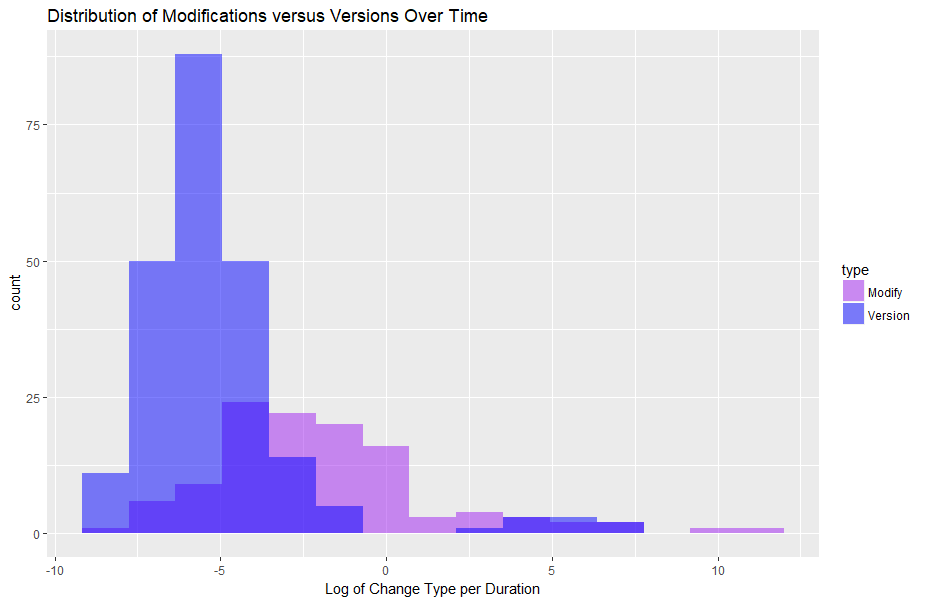
\includegraphics[scale=.6]{figures/Eol_Mod_Ver_Rate.png}
	\caption{Distribution of average normalized Modify counts of each data set in Eath Observing Laboratory.}
	\label{EOL_Mod_Ver}
\end{figure}

\begin{table}
	\caption{Summary of Kolmogorov-Smirnov Test results for Earth Observing Laboratory.}
	\label{table:Eol_KS}
	\centering
	\begin{tabular}{|c|c|c|c|c|}
		\hline
		&	Add&	Invalidate&	Modify&	Versions\\ \hline
		Length&	205&	192&	114&	227\\
		D-Value&	0.12919&	0.14464&	0.19727&	NA\\
		p-Value&	0.05487&	0.02575&	0.005443&	NA\\
		\hline
	\end{tabular}
\end{table}

